\documentclass{article}
\usepackage[utf8]{inputenc}
\usepackage{graphicx}

\title{ISAKMP}
\author{arfritz97 }
\date{August 2019}

\begin{document}

\maketitle

\section {Understanding ISAKMP}

Below is an inital overview of the capabilites of ISAKMP. The procedure for ISAKMP occurs in two phases where phase one is when two entities agree on how to protect further negotiation traffic while negotiating an ISAKMP SA for an authenticated and secure channel. Phase two is when the secure channel is then used to negotiate security services for IPSec.

\begin{itemize}
\item ISAKMP is the protocol for establishing Security Associations (SA) and cryptographic keys in an internet environment.
\item ISAKMP is a part of IKE.
	\begin{itemize}
	\item IKE establishes the shared security policy and authenticated keys.
	\item ISAKMP uses IKE for key exchange.
	\end{itemize}
\item Defines payloads for exchanging key generation and authentication data.
\item Allows an entity's initial communications to indicate which certificate authorities (CAs) it supports.
\item Overall, 4 goals
	\begin{enumerate}
	\item authenticating a communicating peer
	\item creation and management of security associations
	\item key generation techniques
	\item threat mitigation
	\end{enumerate}
\end{itemize}

\section {ISAKMP Header}

\subsection {Header Fields}

\begin{itemize}
\item Initiator Cookie (8 octects) = Cookie of entity that initiated SA establishment, notification, or deletion.
\item Responder Cookie (8 octects) = Cookie of responder 
\item Next Payload (1 octet) = Type of first payload
\item Major/Minor Version (4 bits each) = Version of ISAKMP in use
\item Exchange Type (1 octet) = Type of exchange being used
\item Flags (1 octet) = More stinking flags, encrypt, commit authentication only
\item Message ID (4 octets) = Unique ID to identify things in Phase 2
\item Length (4 octets) = Length of total message (header + payload)
\end{itemize}

\subsection {Next Payload Types}

The following list details the possible next payload types as well as thier associated values.

\begin{itemize}
\item NONE = 0
\item SA = 1
\item Proposal = 2
\item Transofrm = 3
\item Key Exchange = 4
\item Identification = 5
\item Certificate = 6
\item Cert Request = 7
\item Hash = 8
\item Signature = 9
\item Nonce = 10
\item Notification = 11
\item Delete = 12
\item Vendor ID = 13
\item Reserves = 14-127
\item Private Use = 128-225
\end{itemize}

\subsection {Exchange Types}

The next aspect that is necessary to define is the exchange type. This is useful as it tells the responder the desired exchange specifications such as fast exchange or slow exchange. The follow list details the exchange types with their associated values. 

\begin{itemize}
\item NONE = 0
\item Base = 1
\item Id Protection = 2
\item Auth Only = 3
\item Aggressive = 4
\item Informational = 5
\item ISAKMP Future Use = 6 - 31
\item DOI Specific Use = 32 - 127
\item Private Use = 128 - 255
\end{itemize}

\subsection {Payload Headers}

Payload headers can be generic or customized for the situation. A generic header simply includes Payload Data where the Data can change based on the situation. 

\subsection {SA Payload}

The Domain of Interpretation (DOI) and Situation are included in the Security Association payload. Some details about the Domain of Interpretation and Situation can be seen below.

\begin{itemize}
\item DOI (4 octets) = Identifies the DOI under which negotiation takes place. A value of 0 during Phase 1 specifies a Generic ISAKMP SA which can be used for any protocol during Phase 2.
\item Situation = A DOI-specific field that identifies the situation under which this negotiation is taking place. 
\end{itemize}

\subsection {Proposal Payload}

The proposal payload carries many unique aspects as seen with the following list below

\begin{itemize}
\item Payload Length = Length is octets of the entire Proposal payload including the generic payload header, the Proposal payload, and all Transform payloads associated with this proposal.
\item Proposal Number = identifies the proposal number for the current payload
\item Proposal ID = Specifies the protocol identifier such as IPSEC ESP, IPSEC AH, OSPF, TLS, etc.
\item SPI Size = Length in octets of the SPI as defined by the Protocol ID
\item No. of Transforms = Specifies the number of transforms for the proposal.
\item SPI (variable) = sending entity's SPI
\end{itemize}

\subsection {Transform Payload}

The unique thing about transform payloads is they include a Transform Number and a Tranform ID. The Transform number identifies the transform number for the current payload. The Transform ID specifies the transform identifier for the protocol within the current proposal. 

\subsection {Key Exchange Payload}

This payload includes key exchange data which could be of variable length. It is the data required to generate a session key and is specified by the DOI and the associated Key Exchange algorithm.

\subsection {Certificate Payload}

This payload includes cert encoding which indicates the type of certified contained in the certificate field. 

\section {Proposal Syntax}

Perhaps it is most important to understand the composition of a proposal to understand ISAKMP. Proposals with the same Proposal number are taken as a logical AND and Proposals with different numbers are taken as the logical OR. Different transform within a proposal are taken as the logical OR. 

\subsection {Proposal Example}

The following details the chain of communication for this example. 

\begin{itemize}
\item Proposal 1: AH
\item Transform 1: \begin{verbatim}
					HMAC_SHA
					\end{verbatim}	 
\item Transform 2: \begin{verbatim}
					HMAC_MD5
					\end{verbatim}
\item Proposal 2: ESP
\item Transform 1: \begin{verbatim}
					3DES with HMAC-SHA
					\end{verbatim}
\item Transform 2: \begin{verbatim}
					3DES with HMAC-MD5
					\end{verbatim}
\item Transform 3: \begin{verbatim}
					AES with HMAC-SHA-256
					\end{verbatim}
\item Proposal 3: ESP
\item Transform 1: \begin{verbatim}
					3DES with HMAC-SHA
					\end{verbatim}
\item Proposal 4: PCP
\item Transform 1:LZD
\end{itemize}

The base exchange then follows these steps:

\begin{enumerate}
\item The Initiator sends the Header, SA, and Nonce to Responder to begin ISAKMP-SA negotiation
\item The Responder responds with HDR, SA, Nonce resulting in the basic SA being agreed 
\item The Initiator responds with Header, KE, IDii, and Auth which includes the key generated by the responder (KE) and the Initiator identity verified (Idii)
\item The Responder responds with HDR, KE, Idir, Auth which includes the responder ident verified (KE) and the initiator key generated (IDir). The security association (SA) is established. 
\end{enumerate}

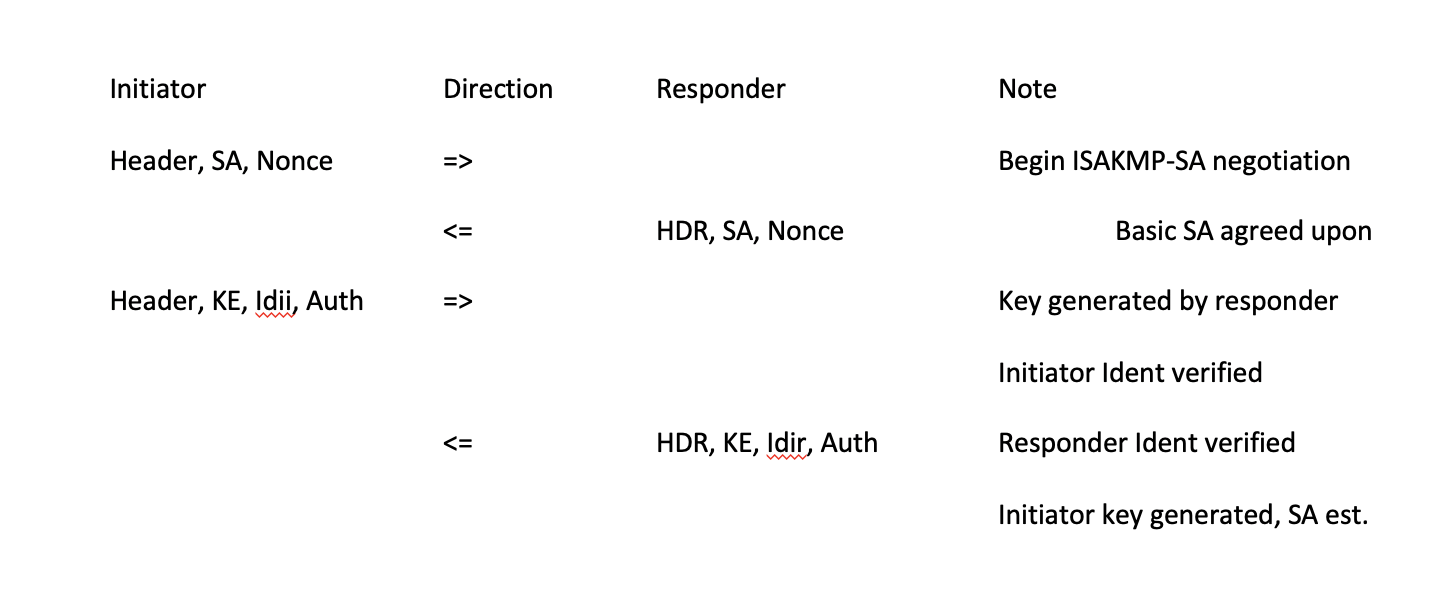
\includegraphics{ISAKMP_Neg_Procedure}



\end{document}
